\section{Versionskontrolle}
\subsection{Versionskontrollsysteme (VCS)}

\begin{multicols}{2}
	\subsubsection{Zweck}
	\begin{itemize}
		\item Aufbewahrung, Verwaltung, Wiederherstellen von Dateien in einem Archiv
		\item Koordination des Zugriffs
	\end{itemize}
	
	\subsubsection{Einsatz}
	\begin{itemize}
		\item Softwareentwicklung
		\item Content-Management-Systeme (CMS)
		\item Archiv $=$ Repository $=$ Lager
	\end{itemize}
\end{multicols}

\subsubsection{Einteilung}
	\begin{itemize}
		\item Lokale Versionskontrollsysteme (LVCS), ein Archiv für jede Datei
		\item Zentralisierte Versionskontrollsysteme (CVCS), ein Archiv für alles
		\item Verteilte Versionskontrollsysteme (DVCS), mehrere verteilte Archive
\end{itemize}

\subsection{Git}
\begin{minipage}{8cm}
\begin{itemize}
	\item Git $\rightarrow$ Blödmann
	\item Entwicklet von Linus Torvalds, Linux-Erfinder
	\item Man arbeitet mittels einer Konsole, kein GUI
	\item Git ist ein DVCS
\end{itemize}
\end{minipage}
\hfill
\begin{minipage}{9cm}
	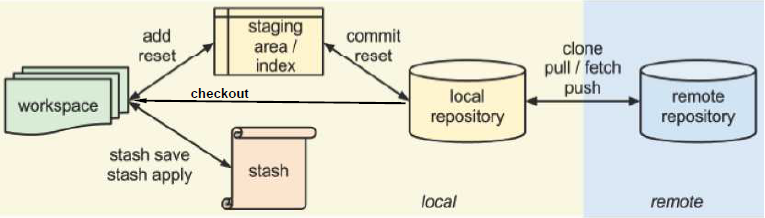
\includegraphics[width=9cm]{images/git.png}
\end{minipage}

\subsubsection{Allgemeines}
\begin{tabular}{|l|l|}
	\hline \textbf{Repository} & Ist ein Archiv für ein Projekt und enthält alle Änderungen und Versionen\\
	\hline \textbf{Branch} & Beschreibt zusammenhängende Änderungen in einem Projekt. Es gibt Minimum einen  bis beliebig viele.\\& Der Master-Branch ist der Produktivzweig\\
	\hline \textbf{Commit} & Beschreibt eine Änderung in einem Branch an einer Datei mit Änderungsinformation\\
	\hline \textbf{Snapshot} & Momentanes Zeitabbild des Projektes\\
	\hline \textbf{Merge} & Zusammenführen von Änderungen aus zwei Branches\\
	\hline \textbf{Stagen} & Datei zum Index hinzufügen\\
	\hline
\end{tabular}
\\
\\
\begin{tabular}{|c|c|}
	\hline \textbf{Lifecycle von Dateien} & \textbf{Branch}\\
	\hline \tabbild[width=9cm]{images/git_lifecycle.png} & \tabbild[width=9cm]{images/git_branch.png}\\
	\hline
\end{tabular}

\subsubsection{Datenbereiche}
\begin{tabular}{|l|l|}
	\hline
	\begin{tabular}[c]{@{}l@{}}\textbf{Workspace}\\ -Projektverzeichniss\\ -hier wird gearbeitet\end{tabular}   & \begin{tabular}[c]{@{}l@{}}\textbf{Repository}\\ -Versionsgeschichte in Form von Commits (Revision)\\ -lokal/remote\end{tabular}   \\ \hline
	\begin{tabular}[c]{@{}l@{}}\textbf{Stash}\\ -Lager\\ -temporäres Speichern der Workspace-Daten\end{tabular} & \begin{tabular}[c]{@{}l@{}}\textbf{Staging Area/Index/Cache}\\ -sammelt Änderungen für Commits\\ -Bereitstellungsraum\end{tabular} \\ \hline
\end{tabular}

\subsubsection{Git-Konzepte}
\begin{itemize}
	\item Git-Workspace ist ein Verzeichnis welches die zu bearbeitenden Dateien eines Projektes enthält
	\item In diesem Verzeichnis ist ein Unterverzeichnis \textit{".git"}
	\item Dieses Unterverzeichnis \textit{".git"} bildet das lokale Repository
	\item Im Branch zeigen die Pointer immer auf den vorhergehenden Commit
	\item Jeder Commit bekommt einen speziellen Hashwert
\end{itemize}